\section{North-East-Down (NED)}\label{sec:ned}

\paragraph{} The North-East-Down is a geographical coordinate system fixed to the Earth's surface, and, precesily because of this, is also known as \textbf{local tangent plane (LTP)} or ground coordinate system (green lines in Figure \ref{fig:Geodetic1}). The origin and axis of this system are defined as follows: 
\begin{itemize}
\item{The origin (\textbf{$O_{n}$}) is located at a arbitrary point on the Earth's surface.}
\item{The X-axis (\textbf{$X_{n}$}) points towards the geodetic north.}
\item{The Y-axis (\textbf{$Y_{n}$}) points towards the geodetic east.}
\item{The Z-axis (\textbf{$Z_{n}$}) points downard along the ellipsoidal normal, set by the right-hand rule.}
\end{itemize}

\paragraph{} The local NED frame plays a very important role in flight control and navigation.
Navigation of small-scale UAVs is normally carried out within this frame. It will later be shown that during this work 2 different local NED frames would be described. One being with the origin fixed at the Ground Station location and one with an origin at the center of gravity of the drone at all times. This is the so-called \textbf{Vehicle-carried NED}.

\begin{figure}[H]
   \centering
    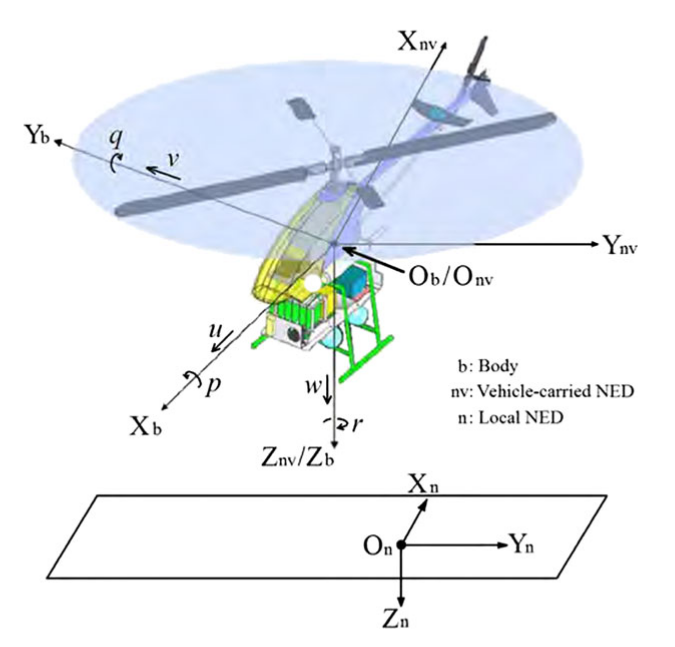
\includegraphics[width=.70\textwidth]{figures/NEDtemp1.png} 
    \caption{Geodetic, ECEF and local NED Frames.}  
    \label{fig:Geodetic1}
\end{figure}

\paragraph{} In mathematics, a spherical coordinate system is a coordinate system for three-dimensional space where the position of a point is specified by three numbers: the \textbf{radial distance} of that point from a fixed origin ($\rho$), its \textbf{polar angle} measured from a fixed zenith direction ($\theta$), and the \textbf{elevation angle} of its orthogonal projection on a reference plane, measured from a fixed reference direction on that plane ($\phi$).

It is necessary to define a unique set of spherical coordinates for each point, and therefore restricting their range is required. In our case the coordinates will be limited as follows:
\begin{align*}
& \rho \geq 0 \\
& -\pi \leq \theta < \pi \\
& \frac{-\pi}{2} \leq \phi \leq \frac{\pi}{2}
\label{eq:los_distToHorizon}
\end{align*} 

\begin{figure}[H]
   \centering
    \includestandalone[width=.50\textwidth]{figures/3D_Sphcoord} 
    \label{fig:Spherical1}
    \caption{Spherical Coordinates}
\end{figure}

These constraints define the conversion between Cartesian and Spherical coordinates such that:
\begin{align*}
x &=  \rho\cos\phi\cos\theta  & \rho &= \sqrt{x^{2} + y^{2} + z^{2}} \\
y &= \rho\cos\phi\sin\theta   & \theta &= \text{atan2}\left(\frac{y}{x}\right)\\
z &= \rho\sin\phi       & \phi &=  \text{atan2}\left(\frac{z}{\sqrt{x^2 + y^2}}\right)
\label{eq:los_distToHorizon}
\end{align*} 